%************************************************
\chapter*{Introduction}
\chaptermark{Introduction} %otherwise gets it wrong? But only here!
\label{pt:introduction}
%Ice cream always melts when forgotten on a table. Or, as a physicist might say, it thermalizes, i.e. evolves towards thermal equilibrium. In every day experience, most classical systems thermalize rapidly, like e.g. aforementioned ice cream, that melts in minutes, or ripples on a pond created by a stone's impact, that settle after a few seconds. 
%There are however some rather exotic systems exhibiting anomalously slow thermalization, e.g. so-called spin glasses\cite{edwardsTheorySpinGlasses1975,binderSpinGlassesExperimental1986}. The key aspect hindering thermalization in these spin glasses are random interactions between the spins that makes it very difficult for the system to move between energetically equivalent states. Thus the disorder has essentially frozen out the dynamics and blocks the path to thermal equilibrium.
When pouring some milk into a cup of coffee, one can watch as it rather quickly distributes itself throughout the cup until a homogeneous mixture is reached (cf. \autoref{fig:classical-coffee}). Or, as a physicist might say, the system evolves to \emph{thermal equilibrium}. The reason for this thermalization process can be stated statistically: There are just many more possible configurations where milk and coffee particles are mixed than ones where they are spatially separated, i.e. most microstates are \emph{typical}. Assuming the dynamics explore many different configurations~\footnote{More precisely, the dynamics needs to be \emph{ergodic}.},
%do not preserve the separation explicitly, 
we will thus find the system in a typical microstate most of the time. So, zooming out and taking a macroscopic point of view, the system appears to be in equilibrium. To emphasize: Although there is still on-going dynamics on the microscopic level, the macroscopic state appears to be stationary simply because most microstates exhibit similar macroscopic features. Importantly, this apparent equilibrium state can be described using only a \emph{few macroscopic quantities}, such as the average temperature and the ratio of milk to coffee.
Knowledge of this handful of values allows to compute all other properties of the system simply by averaging over all compatible microscopic configurations without having to know the precise dynamics. Strikingly, most classical systems show thermalization: From small, simple ones like coffee in a cup, over more complex ones such as fridges and engines even up to stellar objects like black holes. This underpins the great predictive power of \emph{statistical mechanics}.
% This gives enormous predictive power, since we can compute properties of the system simply by averaging over all microscopic configurations compatible with the conserved quantities.
%This simple sketch of thermalization holds true for most classical systems and was the result of the foundational work on statistical mechanics by P. Ehrenfest, L. Boltzmann, J. C. Maxwell, J. W. Gibbs and many more.
% In equilibrium, one can make predictions about a systems properties simply by averaging over all (micro-)states the system can take within the constraints of the globally conserved quantities such as total energy, temperature or milk-to-coffee ratio. 
% Indeed, most classical systems prepared out of equilibrium follow the process just sketched  and reach a state of thermal equilibrium which can be described by statistical mechanics.
% Why interesting?
% Can make predictions of equilibrium properties just be averaging states that are compatible with the few macroscopic parameters.

% Since statistical mechanics is a very powerful tool, it is important to understand its exceptions. One such exception are so-called spin-glasses, i.e. systems of classical dipoles where the interaction strength among them is randomly distributed but fixed~\cite{edwardsTheorySpinGlasses1975,sherringtonSolvableModelSpinGlass1975,binderSpinGlassesExperimental1986}. It has been shown that below a certain temperature, these systems don't reach an equilibrium state. The reason behind this failure of thermalization lies within the randomness: While there are many states of similar energy, these are separated by states of high energy. Thus, once the temperature is too low, the system cannot transition between all energetically allowed states anymore which breaks one of the core assumption of statistical mechanics called ergodicity. 

\begin{figure}[hbt]
	\centering
	\hfil
	\raisebox{-0.5\height}{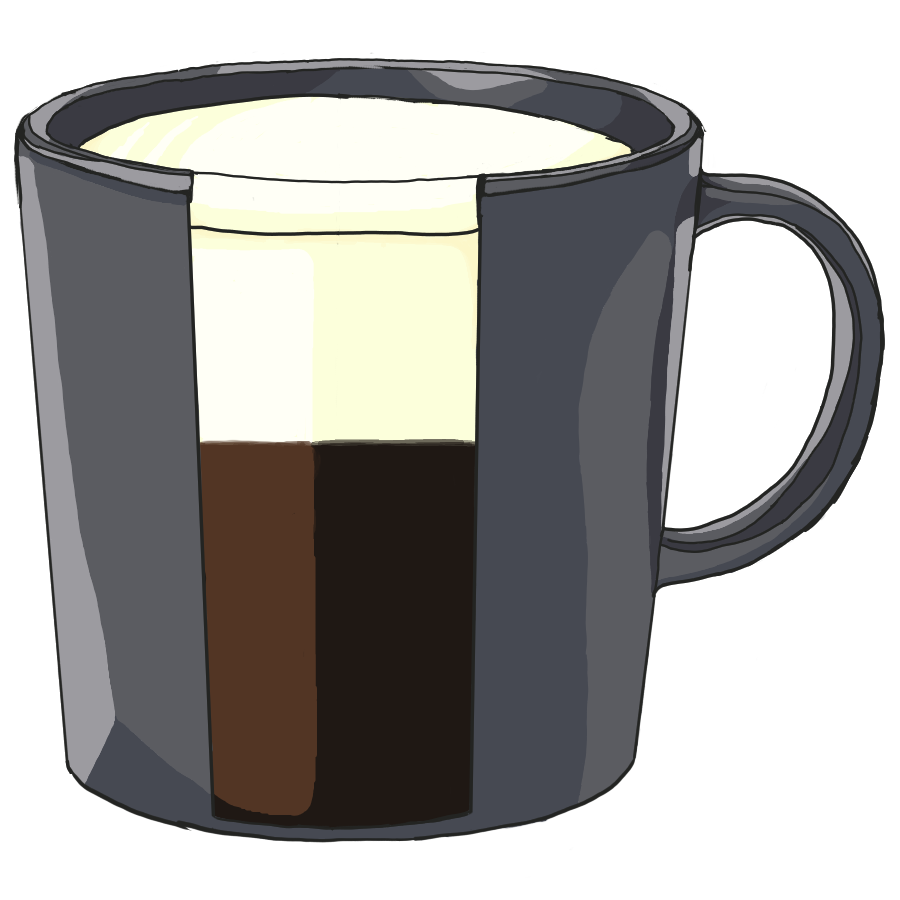
\includegraphics[width=0.3\textwidth]{gfx/intro/Kaffeetasse_C1.png}}
	\hfil
	\raisebox{-0.5\height}{\scalebox{4}{$\longrightarrow$}}
	\hfil
	\raisebox{-0.5\height}{
\includegraphics[width=0.3\textwidth]{gfx/intro/Kaffeetasse_C2.png}}
	\hfil
	\caption{Schematic of the thermalization process of a classical latte.}
	\label{fig:classical-coffee}
\end{figure}

In the quantum realm, the situation turns out to be similar for many cases. For example, even isolated quantum systems initialized in a pure state are oftentimes found to thermalize rapidly. This means they reach a state where observables are consistent with a thermal description depending only on few parameters. This is quite surprising considering the time evolution dictated by the Schrödinger equation preserves the purity and additionally thermal states are usually highly mixed (i.e. a statistical mixture of many pure states). 
Thus an initially pure quantum state can never come close to a thermal state in state space. 
This conundrum can be alleviated by restricting to \emph{local observables}, i.e. observables that extract information from only a small subsystem such as the magnetization of a single spin. Then the measurement process effectively averages over the state of the rest of the system which is equivalent to performing a measurement on a mixed state. 
If most of the states one averages over have the same local expectation value, then this explains the observed thermalization. This assumption is now known as \emph{eigenstate thermalization hypothesis} (ETH)~\cite{deutschQuantumStatisticalMechanics1991,srednickiChaosQuantumThermalization1994, deutschEigenstateThermalizationHypothesis2018} and is conceptually similar to the \emph{typicality} of microstates in classical systems.
%Put in simple terms, ETH guarantees the thermalization of local observables, i.e. observables that only extract information on a small subsystems such as the magnetization of a spin, by putting assertions on the system's spectral properties (cf. Sec.~\ref{sec:Thermalization-in-closed-QS} for the details). 
From a dynamical perspective, the consequences of ETH and thus the mechanism behind quantum thermalization, can be stated more intuitively: Consider some quantum spin system initialized in a product state, such that each spin has a well defined magnetization and there is no entanglement among spins. Letting the system evolve for some time, the interactions will cause entanglement to form and thus the initially local information about the initial state of each spin will be distributed throughout the whole system - hidden in the complicated correlations between all spins and utterly inaccessible to small scale measurements. In fact, 
%a local measurement on such a highly entangled system is akin to performing a measurement on a statistical mixture of systems. 
the stronger the entanglement between subsystem and rest, the more the subsystem appears to be mixed.
Thus the \emph{rapid buildup of entanglement} is the main driver behind thermalization of local observables in closed quantum systems.

% Loosely speaking, ETH asserts that the \emph{individual eigenstates} of the system already look thermal for local observables in the sense that the expectation values match those of a thermal state (cf. Sec.~\ref{sec:Thermalization-in-closed-QS}). %remove spectral description here?

%% Now disordered systems
If interactions are the main reason behind the build-up of entanglement and thus thermalization, shouldn't every non-integrable quantum system thermalize? The story is not as simple as that! 
%While it is true that there are many interacting quantum many-body systems that (at least seem to thermalize)~\cite{rigolThermalizationItsMechanism2008,nandkishoreManyBodyLocalizationThermalization2015,abaninManybodyLocalizationThermalization2019}, there are also a lot of systems in which the nature of their late time behavior is currently hotly debated. Among these are strongly disordered spin systems, where the disorder usually takes the form of random on-site potentials and/or random inter-spin couplings~\cite{andersonAbsenceDiffusionCertain1958,imbrieReviewLocalIntegrals2017,abaninRecentProgressManybody2017,parameswaranEigenstatePhaseTransitions2017,laflorencieEntanglementEntropyLocalization2022}. These disordered systems arise quite naturally in many different contexts such as cold atomic gases~\cite{schreiberObservationManybodyLocalization2015,kondovDisorderInducedLocalizationStrongly2015}, color centers in diamond~\cite{kucskoCriticalThermalizationDisordered2018,martinControllingLocalThermalization2023} or generally systems with impurities~\cite{weiExploringLocalizationNuclear2018,silevitchTuningHighQNonlinear2019}.
In his seminal 1958 paper~\cite{andersonAbsenceDiffusionCertain1958}, Anderson showed that for a single excitation hopping in a lattice with random on-site potentials, all motion, and thus thermalization, arrests \emph{completely} if the randomness of said potentials is sufficiently strong.
This phenomenon, now dubbed Anderson localization, started a new branch of research on models subject to \emph{static randomness}. These kinds of systems arise naturally in many different contexts such as cold atomic gases~\cite{schreiberObservationManybodyLocalization2015,kondovDisorderInducedLocalizationStrongly2015}, color centers in diamond~\cite{kucskoCriticalThermalizationDisordered2018,martinControllingLocalThermalization2023} or generally systems with impurities~\cite{weiExploringLocalizationNuclear2018,silevitchTuningHighQNonlinear2019}. A few years after Anderson's paper, localization was generalized to interacting many-body systems under the name \emph{many-body localization} (MBL)~\cite{fleishmanInteractionsAndersonTransition1980,baskoMetalinsulatorTransitionWeakly2006,gornyiInteractingElectronsDisordered2005,bauerAreaLawsManybody2013}. Conceptually, in an MBL system, the disorder causes local energy mismatches of such severity that the transport of physical quantities (e.g. magnetization) is (almost) completely prohibited~\cite{serbynLocalConservationLaws2013,husePhenomenologyFullyManybodylocalized2014,imbrieReviewLocalIntegrals2017}. So, even though the system appears to be fully interacting at first glance, the strong disorder causes it to fracture into small pieces, called local integrals of motion (LIOMs), that cannot exchange information. Such a system of course \emph{never thermalizes}, so no thermal description can ever be applied! Fortunately, one can still describe the state of the system rather easily if the structure of those LIOMs constituting the system is known. Thus the concept of MBL can also be a practical tool to understand the dynamics of strongly disordered quantum systems.

% MBL does not exist: avanlance thermalization/resonances -> long-range system with resonance counting -> 
The existence of MBL was demonstrated numerically in a large variety of systems with tens of spins/sites in a huge number of studies (e.g.~\cite{palManybodyLocalizationPhase2010,iyerManyBodyLocalizationQuasiperiodic2013,luitzManybodyLocalizationEdge2015,schifferManybodyLocalizationSpin2019,chandaManybodyLocalizationTransition2020})and also experimentally~\cite{schreiberObservationManybodyLocalization2015,choiObservationDiscreteTimecrystalline2017,lukinProbingEntanglementManybody2019,rispoliQuantumCriticalBehaviour2019}. However, its existence in the \emph{thermodynamic limit}, i.e. infinitely large systems, is currently hotly debated~\cite{abaninDistinguishingLocalizationChaos2021,morningstarAvalanchesManybodyResonances2022,haManyBodyResonancesAvalanche2023,scoccoThermalizationPropagationFront2024}. The reason for the absence of MBL in large systems is seen in the so-called \emph{avalanche instability} of MBL~\cite{ponteThermalInclusionsHow2017,thieryManyBodyDelocalizationQuantum2018,crowleyAvalancheInducedCoexisting2020,morningstarAvalanchesManybodyResonances2022}. This mechanism is rooted in the observation that a thermal region can thermalize neighboring LIOMs which results in a larger thermal region. Thus a small thermal inclusion in an otherwise localized system can grow slowly and cause thermalization of the whole. Large enough systems will always feature some statistically \emph{rare regions} of low disorder that then seed a thermalization avalanche.
For systems featuring long-range interactions, which are of particular relevance in this thesis, there exists even more direct arguments based on \emph{counting resonances} that rules out MBL whenever the interaction decays slower then a power-law with exponent twice the spatial dimension~\cite{burinEnergyDelocalizationStrongly2006,yaoManyBodyLocalizationDipolar2014,burinManybodyDelocalizationStrongly2015,burinLocalizationRandomXY2015}.

However, thermalization achieved through either mechanism, avalanche thermalization or resonance proliferation, appears to slowdown exponentially with the system's size~\cite{gopalakrishnanInstabilityManybodyLocalized2019,nandkishoreCriticalLocalizationVan2022,scoccoThermalizationPropagationFront2024}. So it is unproven whether they truly prohibit localization in infinitely large systems. Independently of the theoretical debate, it is unclear how relevant the resulting thermalization timescales are for experiments~\cite{longPhenomenologyPrethermalManyBody2023}. 
In fact in \autoref{ch:experimental-pairs}, we show evidence that MBL can still be applied to describe the dynamics of an experiment featuring power-law interactions with an exponent equal to the spatial dimension despite MBL being ruled out in that parameter range. Of course the experiment can only probe finite times and thus cannot rule out thermalization at later times. Nonetheless, MBL proves to be a useful concept for understanding the observed phenomena.

Notably, most systems used for studying avalanche thermalization or counting resonances feature random on-site potentials, whereas the experiment realizes a bond-disordered model, i.e. its main source of randomness lies within the interactions between the spins. Thus aforementioned arguments might not apply readily to this kind of system. Usually, bond-disordered models are tackled using real-space renormalization group (RSRG) techniques, which iteratively identify and eliminate the strongest coupling of the system~\cite{igloiStrongDisorderRG2005,parameswaranEigenstatePhaseTransitions2017,igloiStrongDisorderRG2018,monthusStrongDisorderRenormalization2018}. Traditionally, RSRG has been applied to models with nearest neighbor interactions to derive properties of the groundstate (e.g.~\cite{dasguptaLowtemperaturePropertiesRandom1980,fisherRandomTransverseField1992,voskManybodyLocalizationOne2013}) but was recently generalized to study excited states as well~\cite{pekkerHilbertGlassTransitionNew2014}. Even more recently it has also been applied to long-range systems~\cite{moureManyBodyLocalizationTransition2015,moureDisorderedQuantumSpin2018,mohdebEntanglementPropertiesDisordered2020,mohdebExcitedEigenstateEntanglementProperties2022,mohdebGlobalQuenchDynamics2023}. All of these works use exact numerics to benchmark their results and thus comparison is limited to small systems.

Given this background, we explore localization phenomena in \autoref{pt:spatial-disorder} using a model that can be realized naturally in a Rydberg quantum simulator.  This opens up the possibility for benchmarking the theoretical results with much larger systems than accessible via numerics. Concretely, we consider a bond-disordered Heisenberg spin model where the disorder arises from power-law interaction between randomly positioned spins. 
After a brief review of the relevant context in \autoref{ch:concepts-thermalization}, we start the analysis of this model in \autoref{ch:pair-localization-transition} by performing a numerical study in one spatial dimension across disorder strength. We find a clear crossover from a thermalizing into a localized regime at sufficiently strong disorder and apply RSRG to derive the locally (quasi-)conserved quantities, which consist of pairs of strongly interacting spins. In the following \autoref{ch:cTWA-paper}, we show how this emergent structure of the system can be exploited to compute the dynamics efficiently and accurately with a semi-classical numerical technique. Finally in \autoref{ch:experimental-pairs}, we turn to a quantum simulator based on ultra-cold Rydberg atoms, that naturally implements the type of model studied, and present two different experimental studies that show clear signatures of localization based on pairs of spins. 
While this cannot answer the question about the stability of MBL in infinitely large systems at arbitrarily late times, it nonetheless establishes once more that MBL can be a quite useful concept to understand the dynamics of real-world systems effectively.

Shifting focus from closed quantum systems to periodically driven systems, MBL seems to have a stabilizing effect on the dynamics even in the presence of strong driving. Usually driving causes the system to absorb energy from the drive and heat up causing it to evolve into a featureless infinite temperature state. However, if the system exhibits MBL, then the energy absorption can be suppressed and the system can remain perpetually in an out-of-equilibrium state~\cite{abaninTheoryManybodyLocalization2016,elsePrethermalPhasesMatter2017,bordiaPeriodicallyDrivingManyBody2017,elseDiscreteTimeCrystals2020a}. This allows for novel out-of-equilibrium phases of matter to exist that can show radically different properties than regular phases. One such new feature is the spontaneous breaking of time translation symmetry which is normally impossible~\cite{watanabeAbsenceQuantumTime2015}. This broken symmetry manifests as \emph{stable oscillations} of the system that show a different frequency compared to the drive. A state breaking time translation symmetry is called a \emph{time crystal} in analogy to ordinary crystals that break spatial translation symmetry. 

Since this phenomenon seems to be closely linked to disorder as well, in \autoref{pt:floquet} of this thesis, we study two periodically driven systems with unusual spatial inhomogeneity: In Chapter~\ref{ch:metronome-spin}, we consider a spatially varying driving field and find it to dramatically enhance the lifetime of time crystalline signatures in an otherwise clean Ising chain. Following this in Chapter~\ref{ch:rydberg-timecrystal}, we consider again the spatially disordered Heisenberg XXZ model from Part~\ref{pt:spatial-disorder} subject to periodic driving. We show preliminary measurements and undertake a theoretical 
exploration regarding the longevity of this time crystalline behavior based on the pair model.

So this thesis consists of two major parts: \autoref{pt:spatial-disorder} discussing localization in closed quantum systems caused by disorder in the interactions due to spatially random positions. And \autoref{pt:floquet} about the effect of spatial inhomogeneity in the context of Floquet time crystals.
Each part starts with an overview of the relevant concepts (\autoref{ch:concepts-thermalization} and \autoref{ch:introduction-floquet} respectively) and ends with a discussion of the results including directions for future research (\autoref{ch:discussion-pair-localization} and \autoref{ch:floquet-discussion}). This thesis closes in \autoref{pt:summary} with a short, high-level, summary of its findings.

%In this thesis, we study both closed and periodically driven quantum spin systems subject to different forms of spatial disorder. As such this thesis consists of two major parts: 
%In Part~\ref{pt:spatial-disorder}, we explore localization phenomena in a bond-disordered Heisenberg spin model where the disorder arises from power-law interaction between randomly positioned spins. After establishing the relevant context in Chapter~\ref{ch:concepts-thermalization}, we start in Chapter~\ref{ch:pair-localization-transition} by performing a numerical study on the model in one spatial dimension across disorder strength. We find a clear crossover from a thermalizing regime into a localized regime at sufficiently strong disorder and derive the locally (quasi-)conserved quantities, which consist of pairs of strongly interacting spin. In the following Chapter~\ref{ch:cTWA-paper}, we show how this emergent structure of the system can be exploited to compute the dynamics efficiently and accurately with a semi-classical numerical technique. Finally in Chapter~\ref{ch:experimental-pairs}, we turn to a quantum simulator based on ultra-cold Rydberg atoms, that naturally implements the type of model studied, and present two different experimental studies that show clear signatures of localization based on pairs of spins.